\documentclass[xetex,mathsans,sans]{beamer}
\usetheme{Boadilla}
\usecolortheme{orchid}
\usepackage{fontspec}
\setsansfont{Basis Grotesque Pro}
\setbeamertemplate{navigation symbols}{}


\title[NuCypher]{NuCypher: Key-Management System}
\author[Derek]{Derek Pierre, Business Development Lead}
\date[21 Jun 2018]{Cyber @ Station F, 21 Jun 2018}

\begin{document}
    \begin{frame}
        \titlepage
        \begin{figure}
            \centering
            
\includegraphics[width=5cm]{pdf/nucypher_logo.pdf}
        \end{figure}
    \end{frame}

    \begin{frame}
      \frametitle{Problem}
      \framesubtitle{Data Breaches}
        \begin{figure}
            \centering
            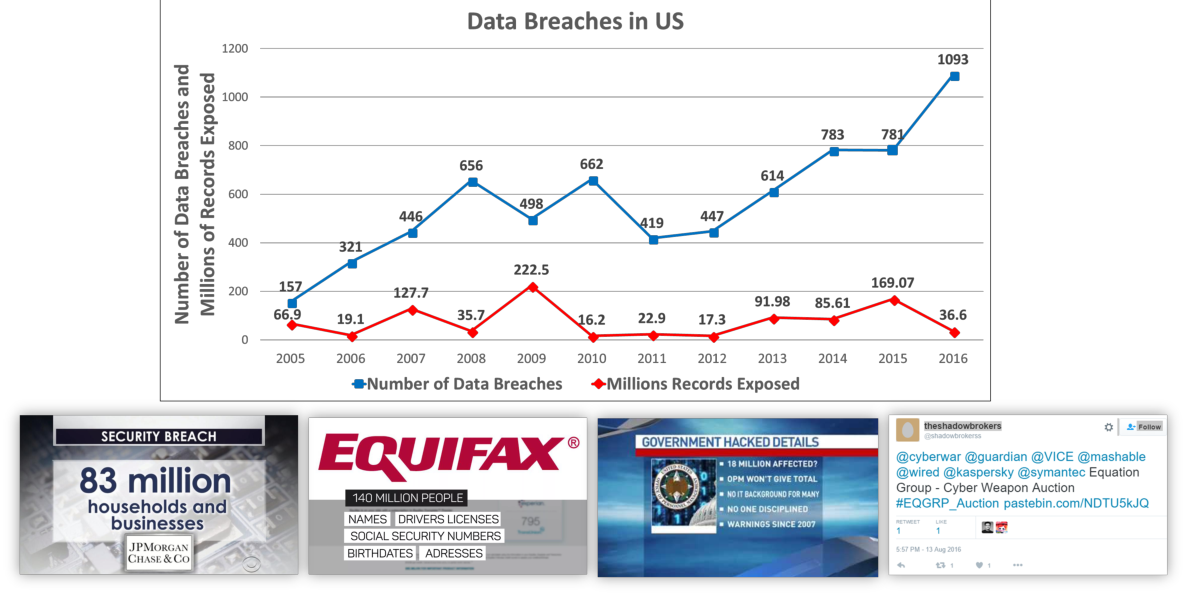
\includegraphics[height=6.5cm]{pdf/data-breaches.pdf}
        \end{figure}

        {\tiny Source: \url{https://www.statista.com/statistics/273550/data-breaches-recorded-in-the-united-states-by-number-of-breaches-and-records-exposed/} \par}
    \end{frame}

    \begin{frame}
        \frametitle{Central Server + TLS}
        \framesubtitle{Data vulnerable to hackers, state actors etc}
        \begin{figure}
            \centering
            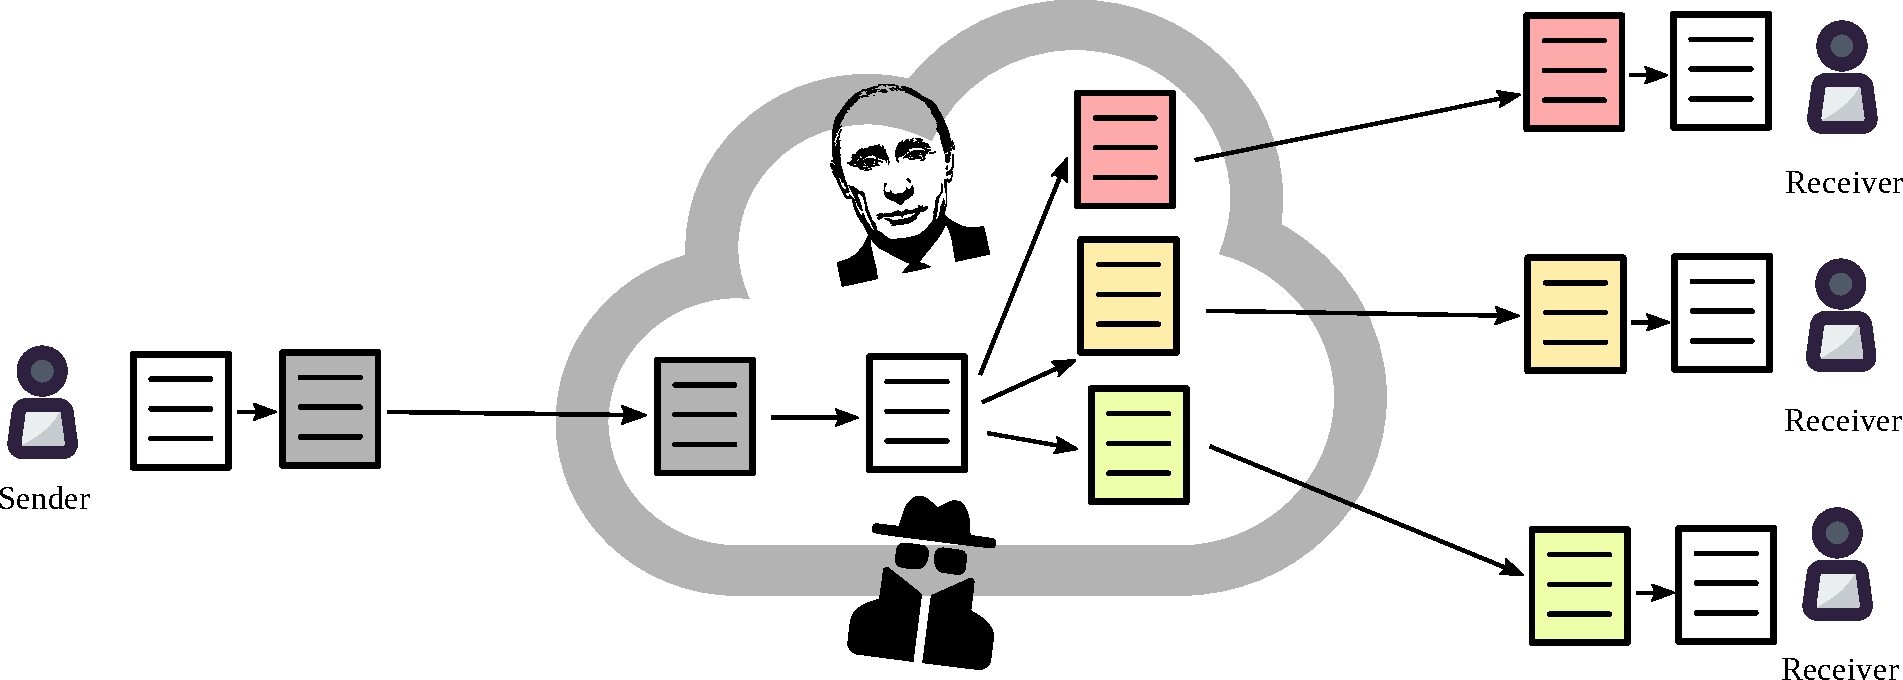
\includegraphics[width=11cm]{pdf/file-sharing-tls.pdf}
        \end{figure}
    \end{frame}

    \begin{frame}
        \frametitle{Public Key Encryption (PKE)}
        \begin{figure}
            \centering
            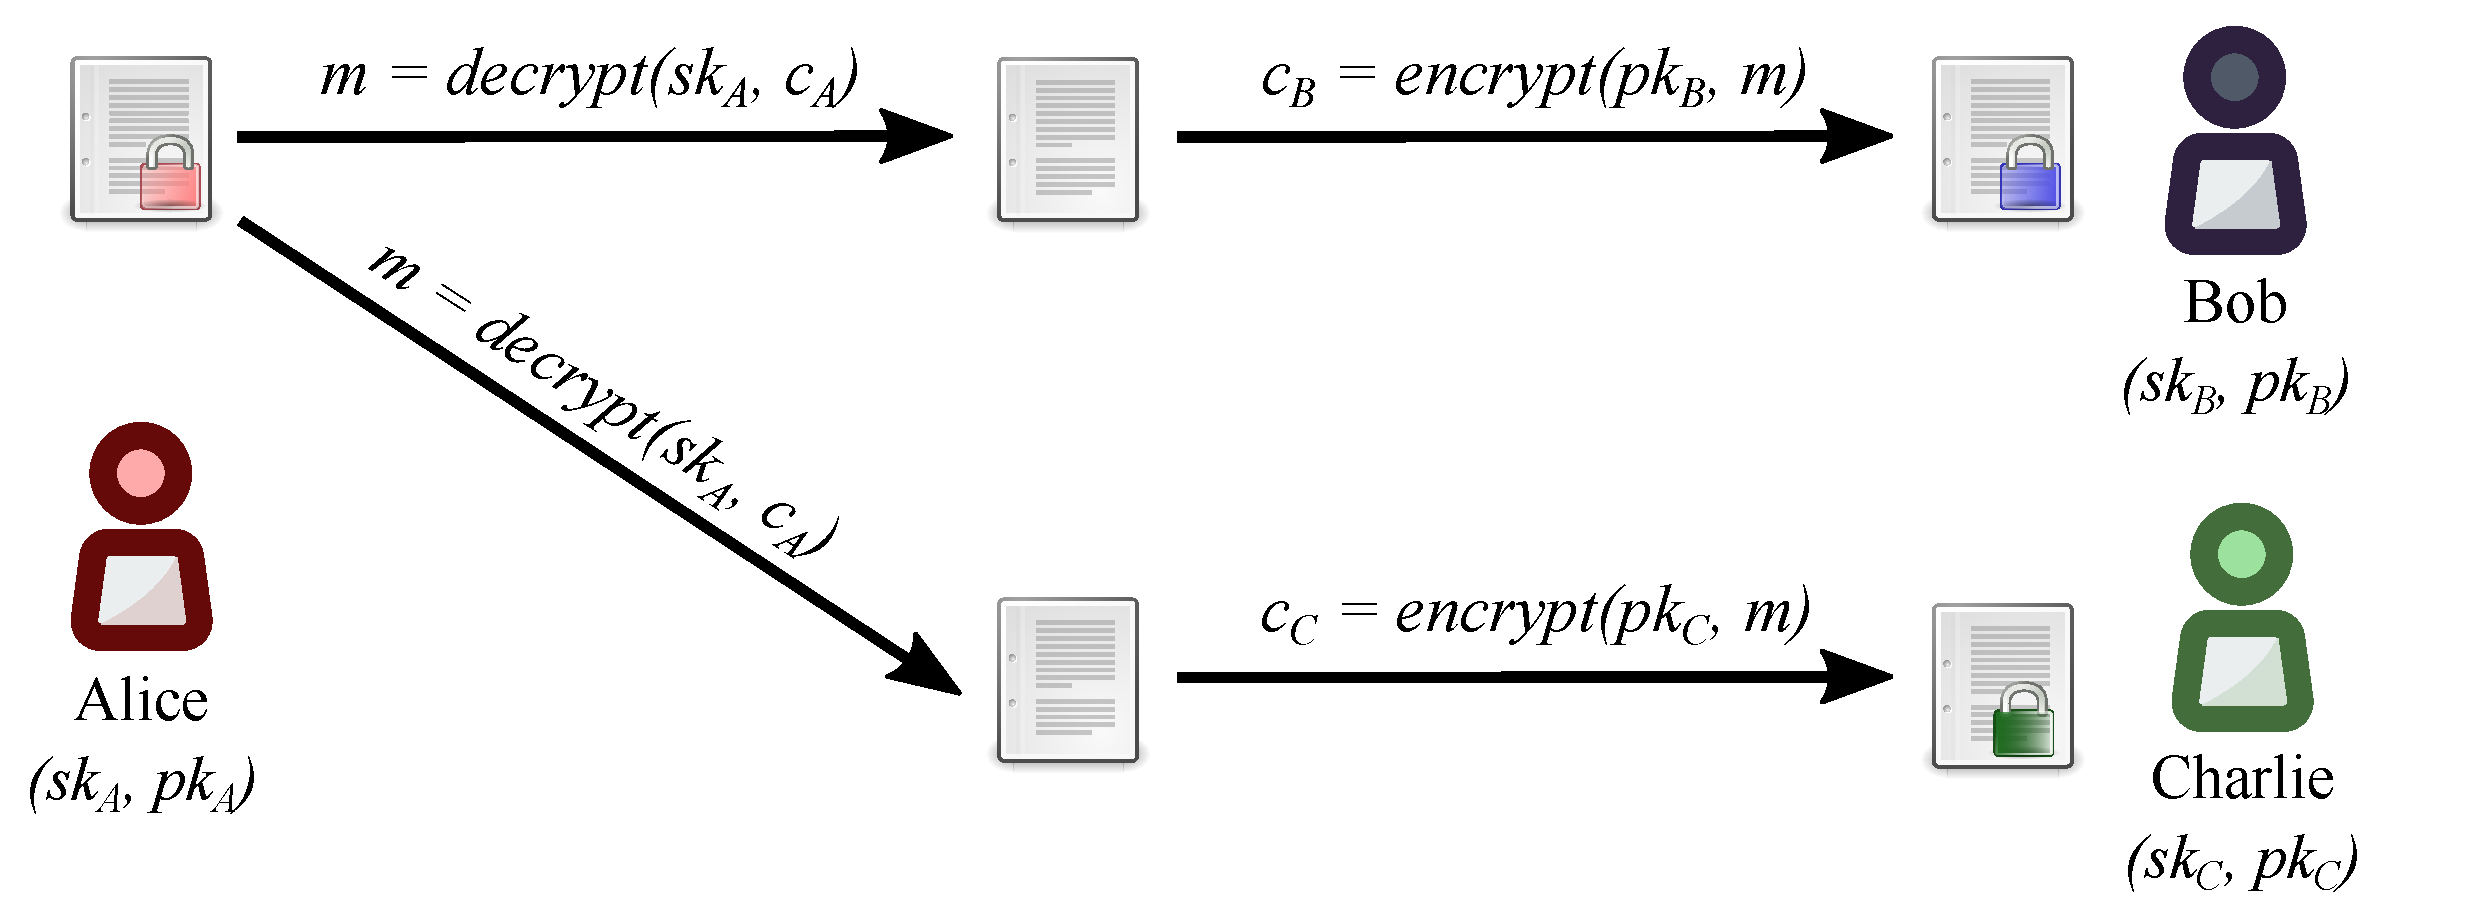
\includegraphics[width=11cm]{pdf/pke.pdf}
        \end{figure}

        Limitations
        \begin{itemize}
            \item Decryption required before sharing
            \item Not scalable
            \item Complex access revocation
        \end{itemize}
    \end{frame}

    \begin{frame}
        \frametitle{What is proxy re-encryption (PRE)}
        \begin{figure}
            \centering
            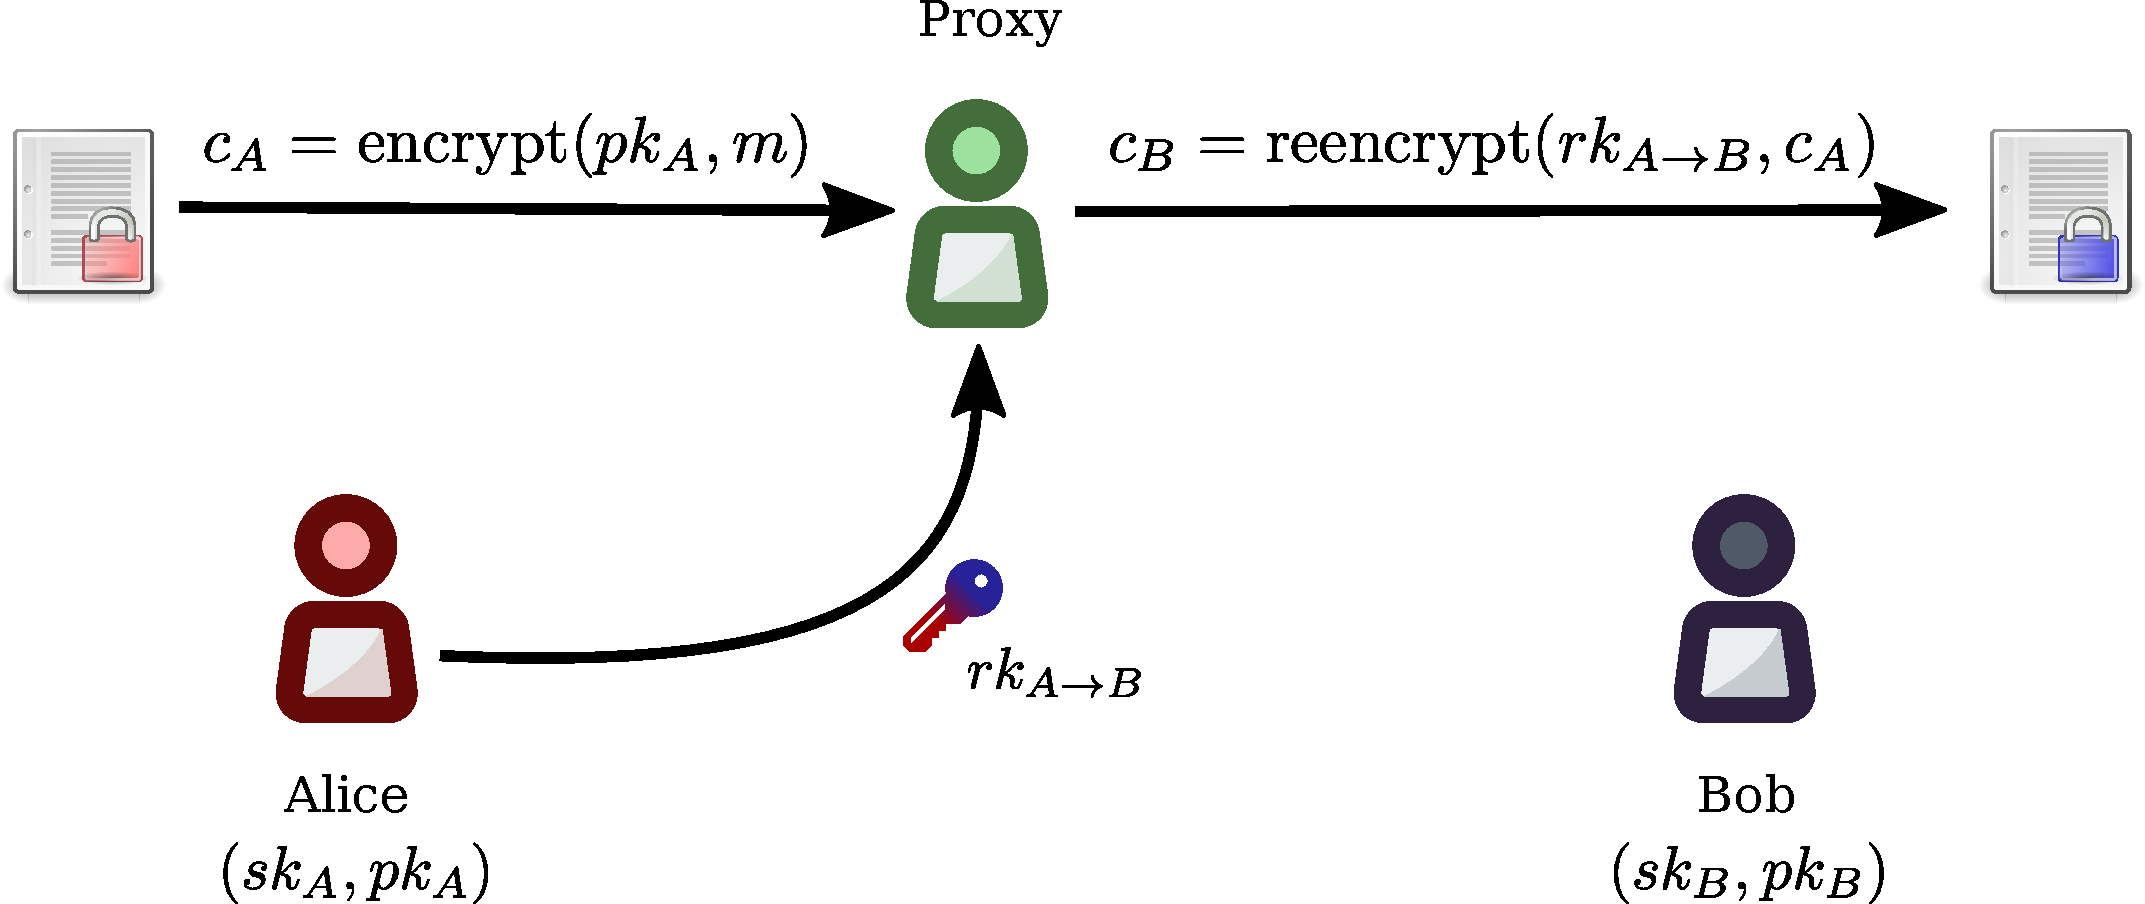
\includegraphics[width=11cm]{pdf/pre.pdf}
        \end{figure}
    \end{frame}

    \begin{frame}
        \frametitle{Solution}
        \framesubtitle{Proxy Re-encryption + KMS}
        \begin{figure}
            \centering
            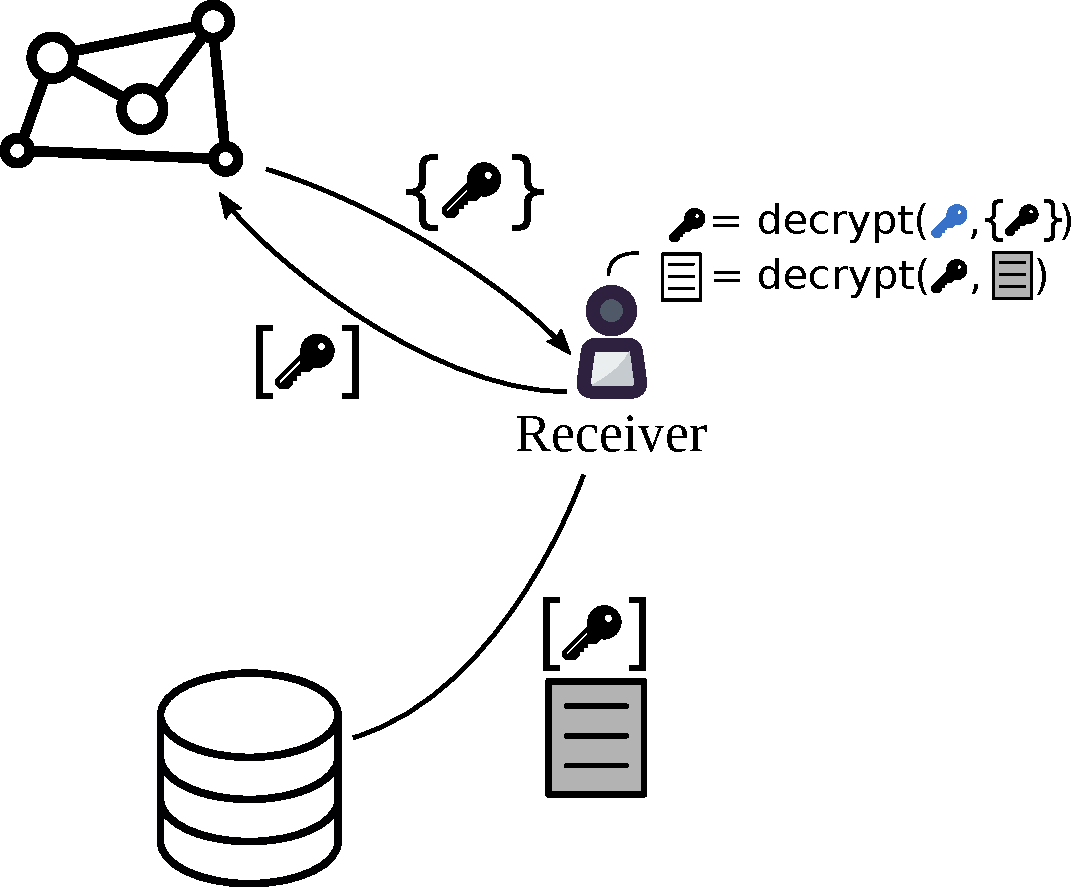
\includegraphics[height=5cm]{pdf/pre-kms.pdf}
        \end{figure}

        Advantages
        \begin{itemize}
            \item Data not decrypted to facilitate sharing
            \item Scalable and performant
            \item Access revocation through re-encryption key deletion
            \item Secure use of data storage providers
        \end{itemize}
    \end{frame}

    \begin{frame}
        \frametitle{Centralized KMS using PRE}
        \framesubtitle{Encryption}
        \begin{figure}
            \centering
            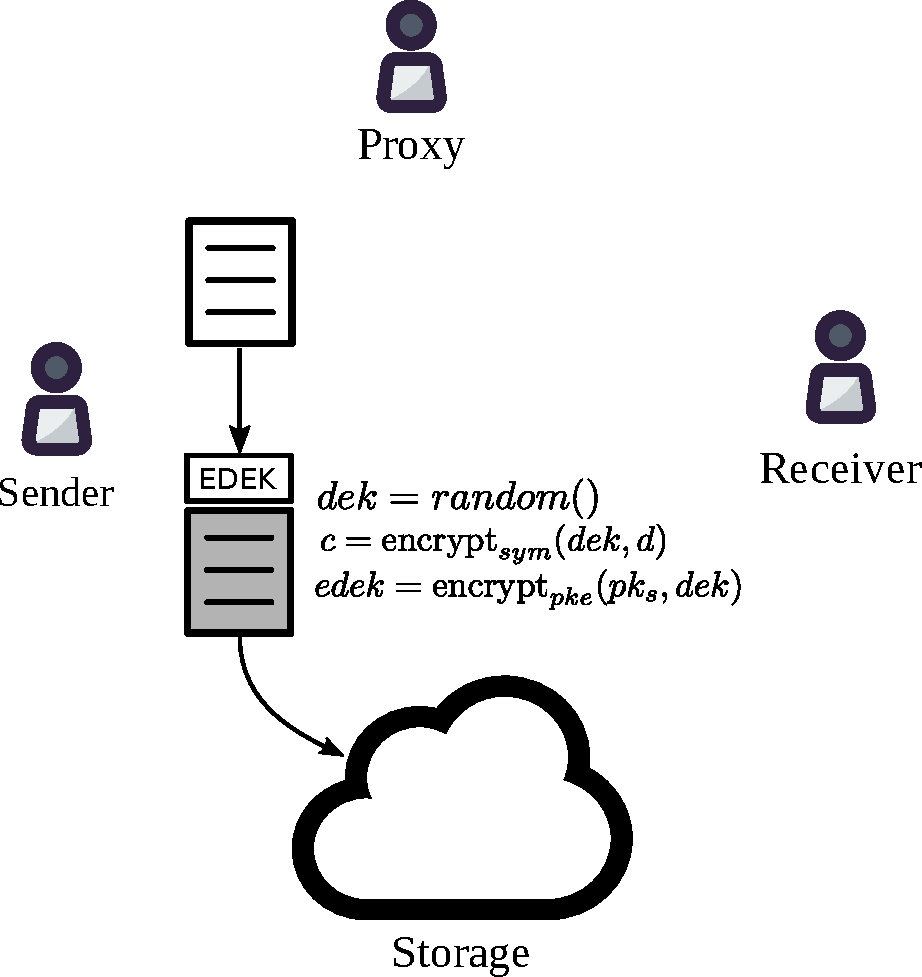
\includegraphics[height=5.5cm]{pdf/encrypt.pdf}
        \end{figure}
    \end{frame}

    \begin{frame}
        \frametitle{Centralized KMS using PRE}
        \framesubtitle{Access delegation}
        \begin{figure}
            \centering
            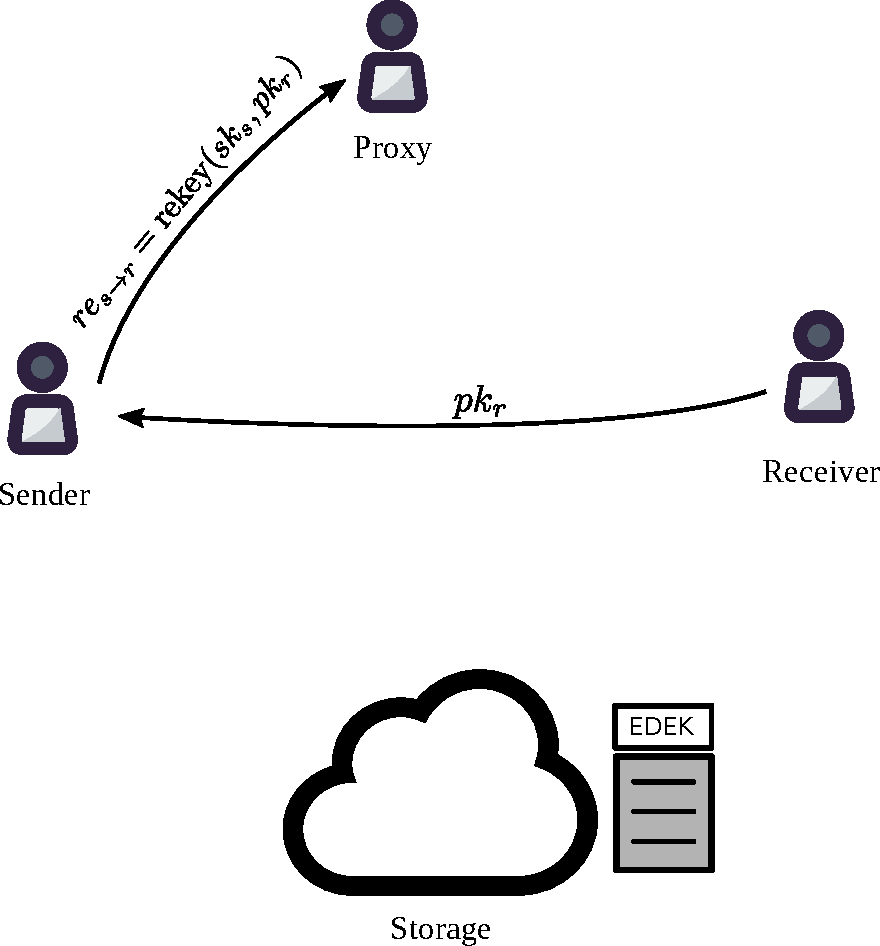
\includegraphics[height=5.5cm]{pdf/delegate.pdf}
        \end{figure}
    \end{frame}

    \begin{frame}
        \frametitle{Centralized KMS using PRE}
        \framesubtitle{Decryption}
        \begin{figure}
            \centering
            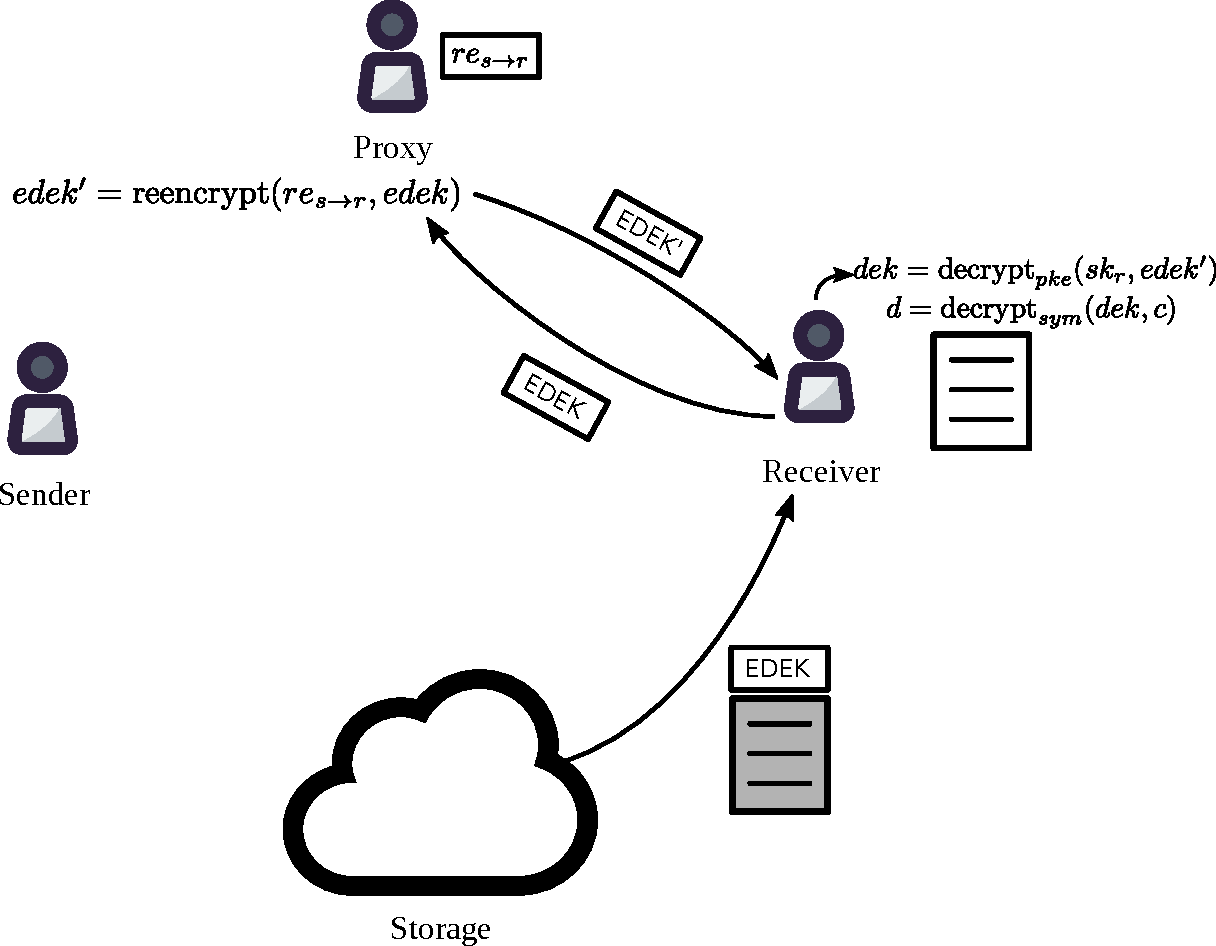
\includegraphics[height=5.5cm]{pdf/decrypt.pdf}
        \end{figure}
    \end{frame}

    \begin{frame}
        \frametitle{Decentralized KMS using PRE}
        \framesubtitle{Using threshold split-key re-encryption (Umbral)}
        \begin{figure}
            \centering
            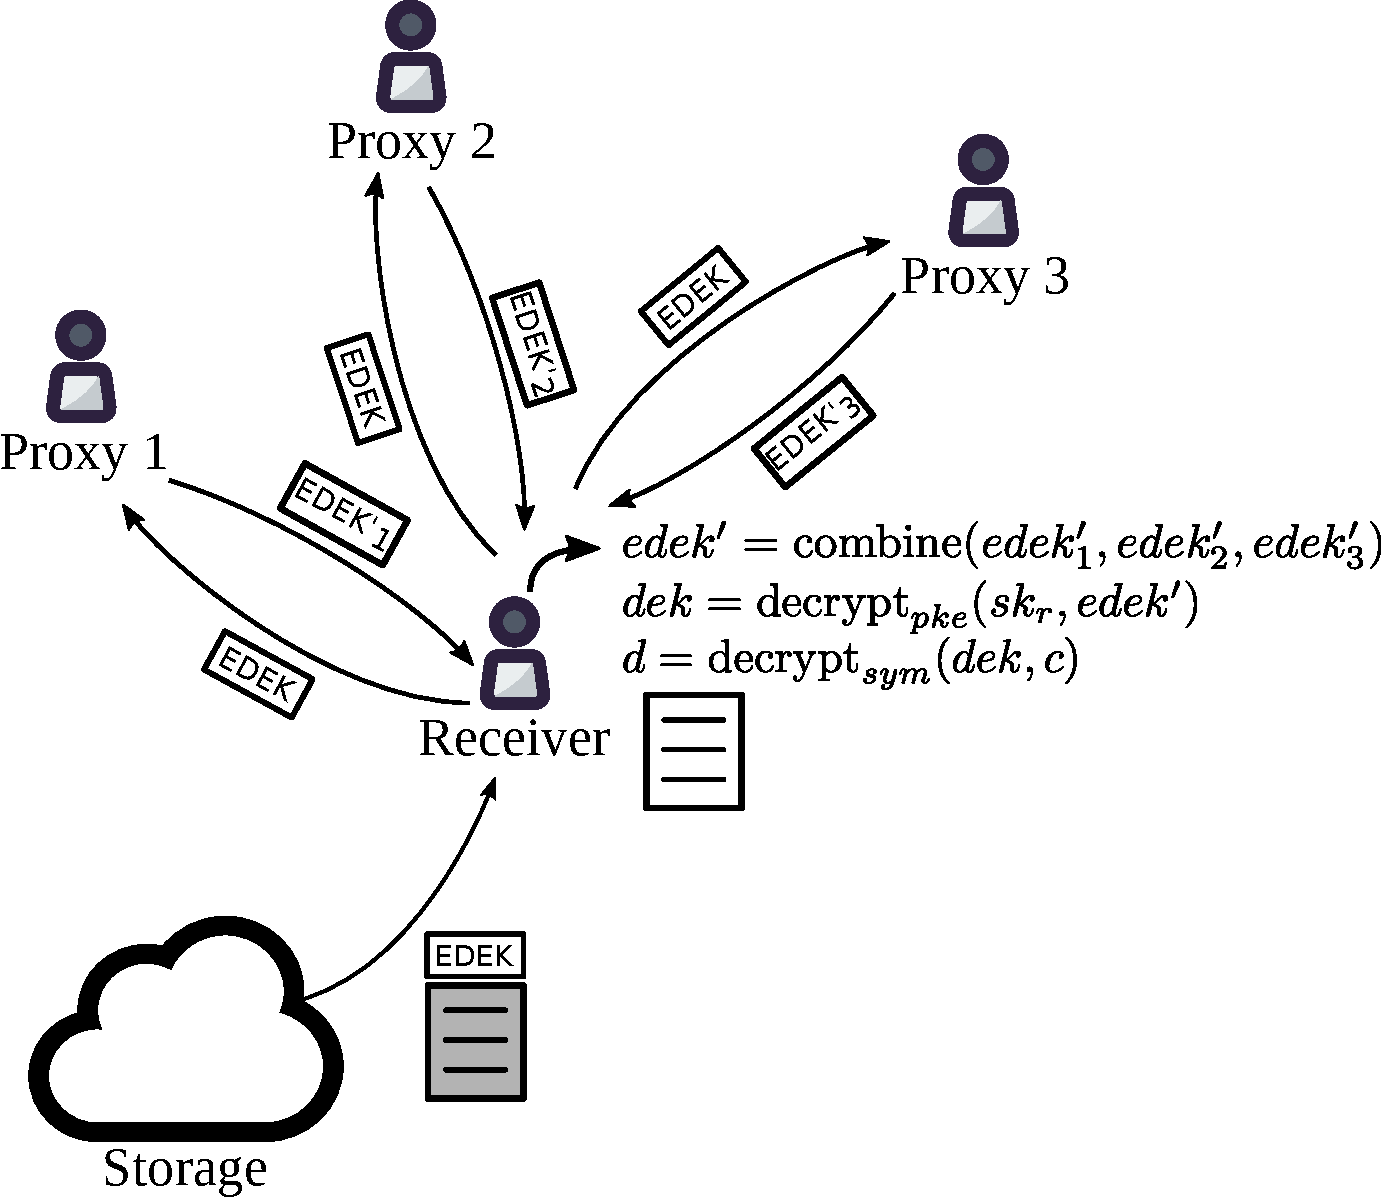
\includegraphics[height=6.5cm]{pdf/decrypt-umbral.pdf}
        \end{figure}
        %\url{https://github.com/nucypher/nucypher-kms/}
        %\url{https://github.com/nucypher/pyUmbral/}
    \end{frame}

    \begin{frame}
        \frametitle{Decentralized KMS: Token}
        \framesubtitle{Purpose}
        \begin{itemize}
            \item Splitting trust between re-encryption nodes (more tokens = more trust and more work)
            \item Proof of Stake for minting new coins according to the mining schedule
            \item Security deposit to be at stake against malicious behavior of nodes
        \end{itemize}
    \end{frame}

    \begin{frame}
        \frametitle{Use Cases}
        \framesubtitle{Multi-tenant, Multi-source Shared Data Lake}
        \begin{figure}
            \centering
            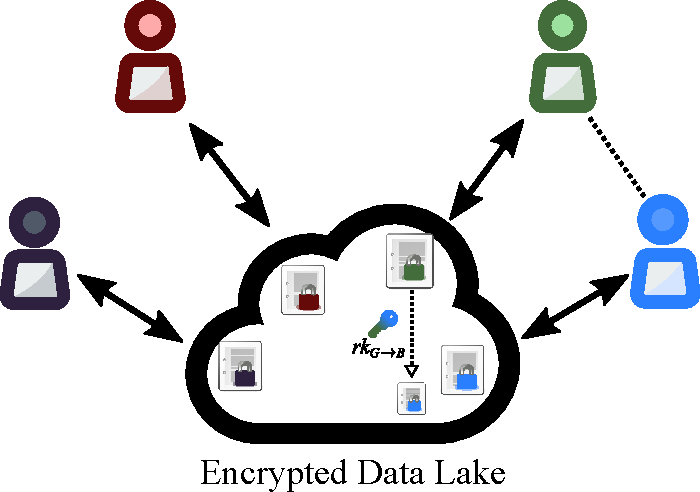
\includegraphics[height=7cm]{pdf/data-lake.pdf}
        \end{figure}
    \end{frame}

    \begin{frame}
        \frametitle{Use Cases}
        \framesubtitle{Encrypted file sharing}
        \begin{figure}
            \centering
            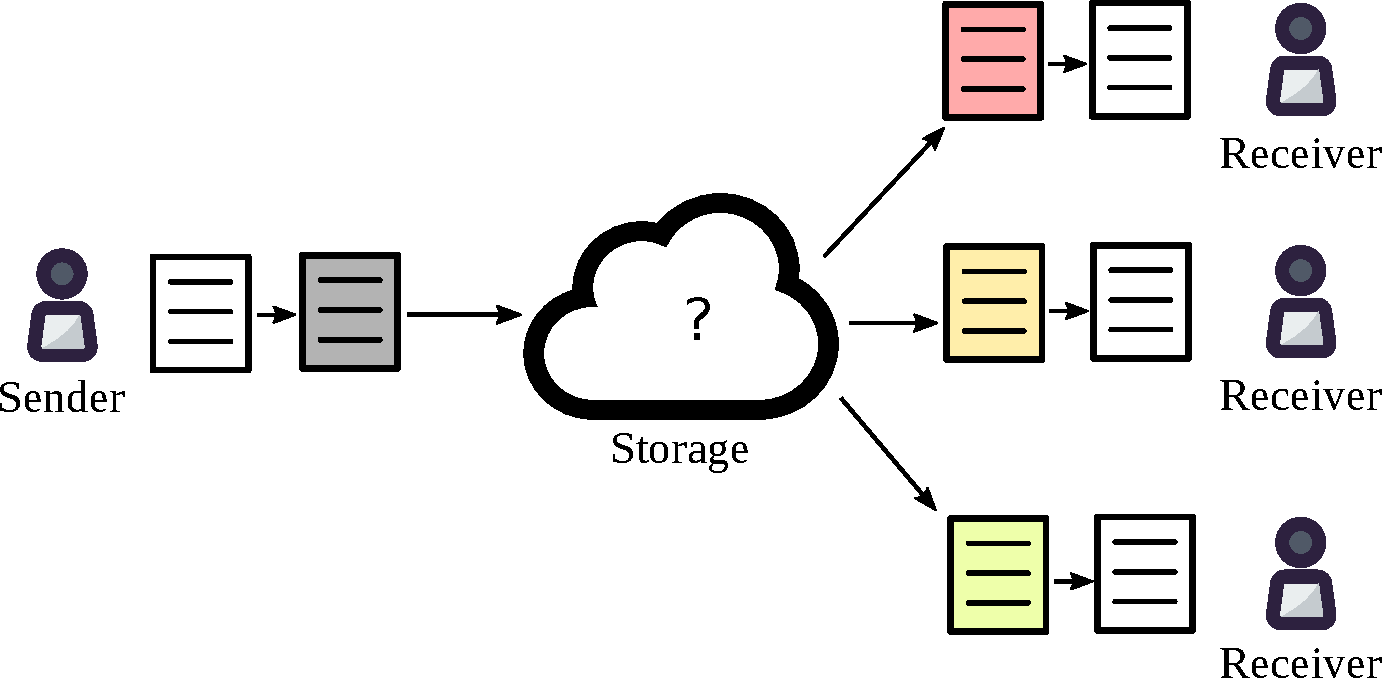
\includegraphics[height=5.5cm]{pdf/file-sharing.pdf}
        \end{figure}
    \end{frame}

    \begin{frame}
        \frametitle{Use Cases}
        \framesubtitle{Encrypted multi-user chats}
        \begin{figure}
            \centering
            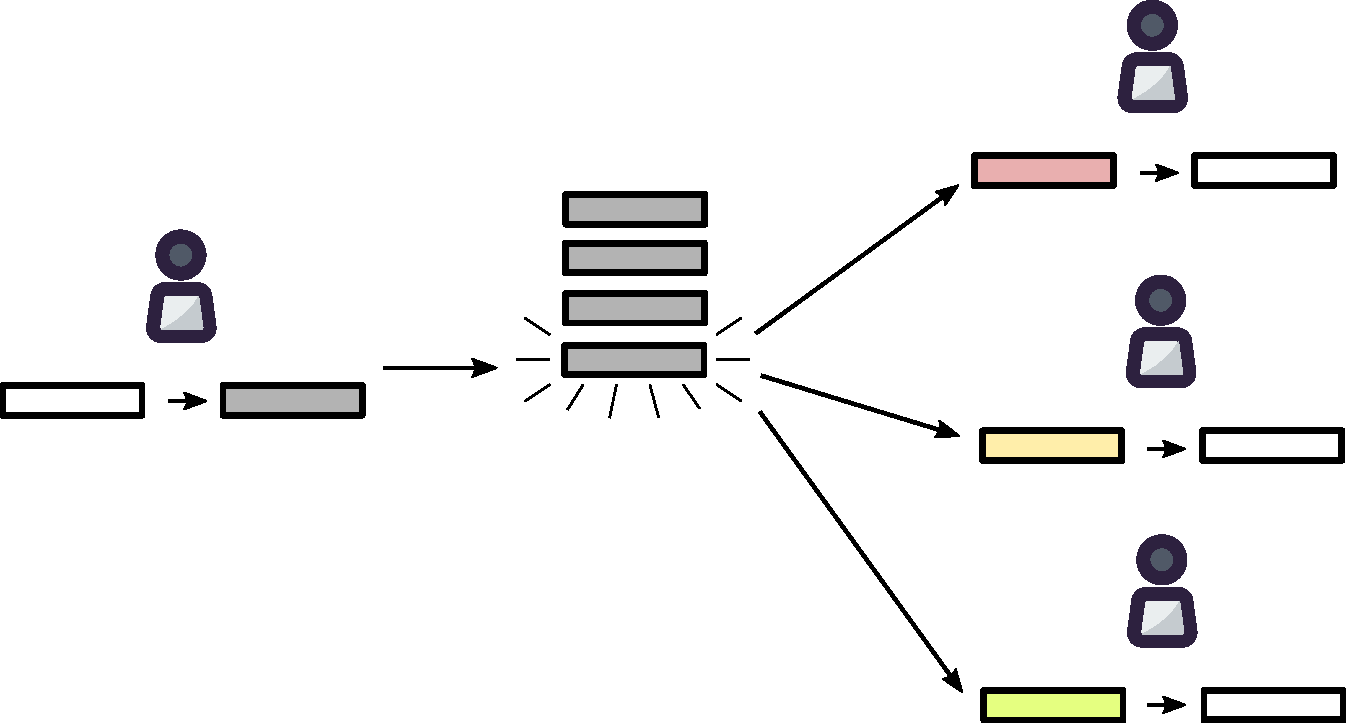
\includegraphics[height=5cm]{pdf/chats.pdf}
        \end{figure}
    \end{frame}

    \begin{frame}
        \frametitle{Use Cases}
        \framesubtitle{Decentralized Access-Controlled Content}
        \begin{figure}
            \centering
            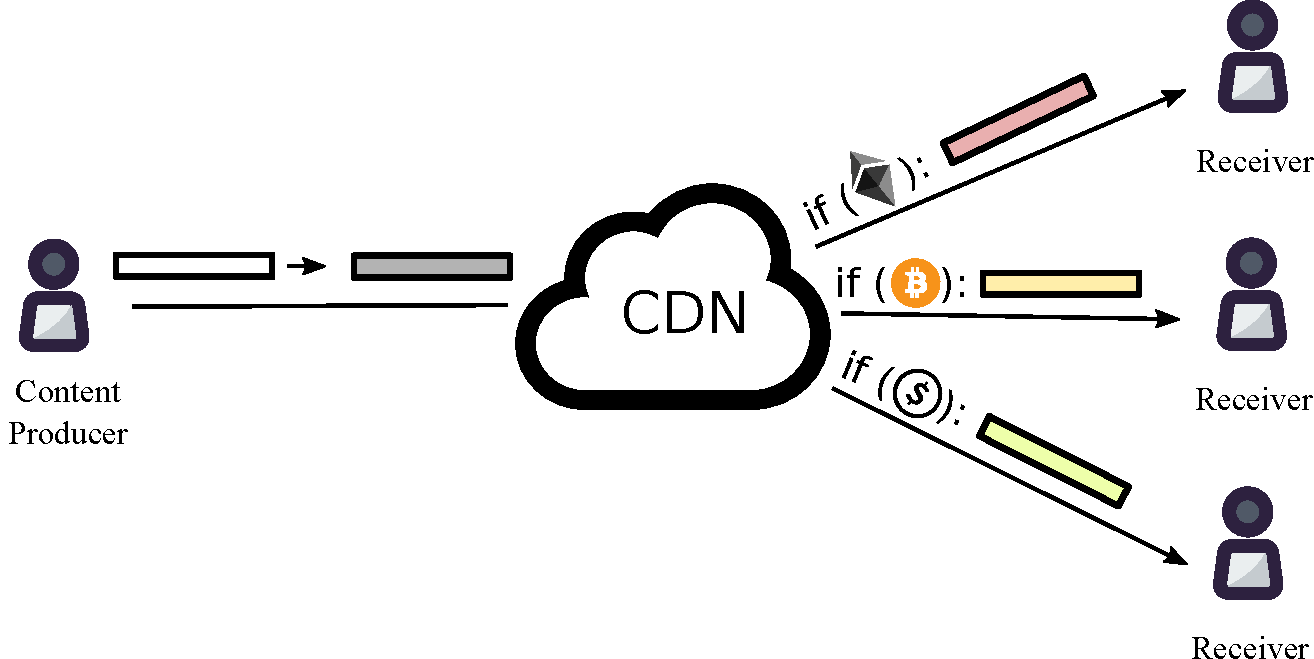
\includegraphics[height=5.5cm]{pdf/content.pdf}
        \end{figure}
    \end{frame}

    \begin{frame}
      \frametitle{Early Users}
      Decentralized marketplaces
      \begin{itemize}
          \item Datum
      \end{itemize}
      Decentralized databases
      \begin{itemize}
          \item Bluzelle
          \item Fluence
          \item Wolk
      \end{itemize}
      Medical data sharing
      \begin{itemize}
          \item Medibloc
          \item IRYO
          \item Medixain
      \end{itemize}
      Other
      \begin {itemize}
          \item Xain [AI]
          \item Origin [Sharing Economy]
          \item Spherity [IoT]
      \end{itemize}
    \end{frame}

    \begin{frame}
      \frametitle{Competing Technology}
       Data Masking and Tokenization
       \begin{itemize}
           \item Less secure for data with underlying patterns
           \item Reduce the value of data by obfuscating it
       \end{itemize}
      
       Fully Homomorphic Encryption
       \begin{itemize}
           \item Slow Peformance
           \begin{itemize}
               \item NuCypher has made investments in this area
           \end{itemize}
       \end{itemize}
       
       Multi-Party Computation
       \begin{itemize}
           \item Slow Performance
       \end{itemize}
     \end{frame}
    
    \begin{frame}
      \frametitle{Investors}
        \begin{figure}
            \centering
            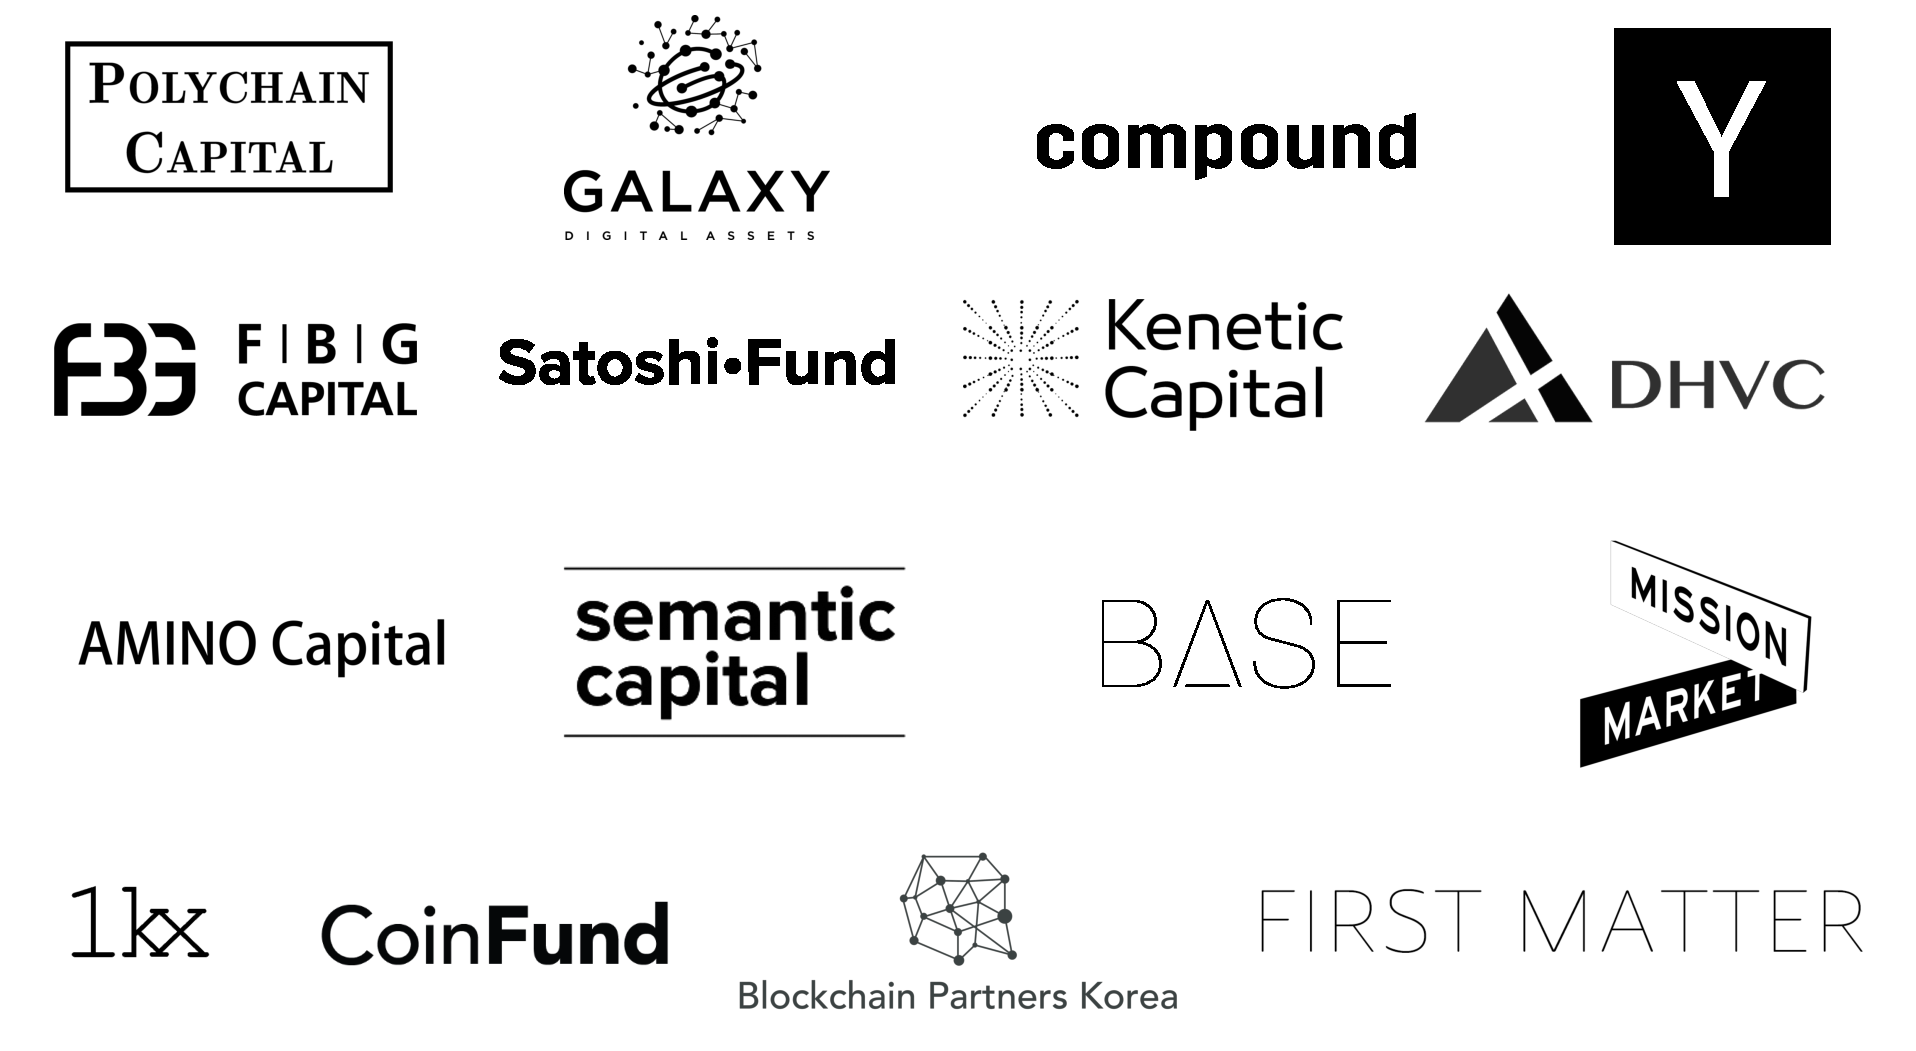
\includegraphics[height=6.5cm]{pdf/investors.pdf}
        \end{figure}
    \end{frame}

    \begin{frame}
      \frametitle{Team}
        Founders
        \begin{figure}
            \centering
            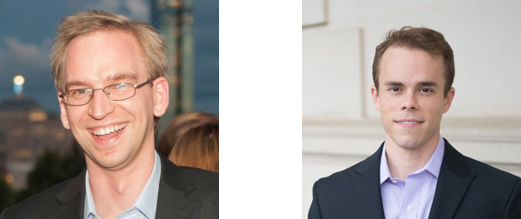
\includegraphics[width=5cm]{pdf/founders.pdf}
        \end{figure}

        Advisors
        \begin{figure}
            \centering
            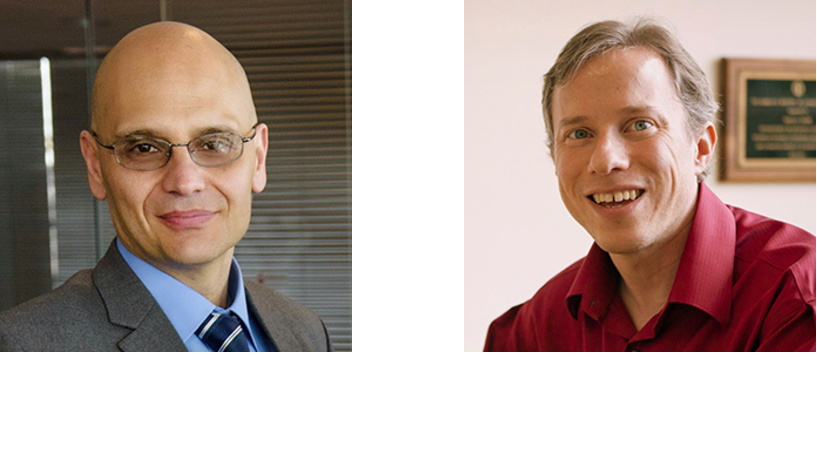
\includegraphics[width=3.5cm]{pdf/advisors.pdf}
        \end{figure}

        9 employees
    \end{frame}

    \begin{frame}
      \frametitle{Why Thales \& Cyber @ Station F}
      \begin{itemize}
          \item Collaboration opportunities for data privacy and compliance
          \item Potential integration with Thales' HSMs
          %\item Grow NuCypher's Enterprise and Cloud business
          \item Expand customer base in Europe
          \item Explore new industry verticals
      \end{itemize}
    \end{frame}

    \begin{frame}
        \frametitle{More Information}
        \begin{figure}
            \centering
            
\includegraphics[width=5cm]{pdf/nucypher_logo.pdf}
        \end{figure}
        Website: \url{https://nucypher.com}

        Whitepaper: \url{https://www.nucypher.com/whitepapers/english.pdf}

        Github: \url{https://github.com/nucypher}

        Discord: \url{https://discord.gg/7rmXa3S}

        Email: \href{mailto:derek@nucypher.com}{derek@nucypher.com}
    \end{frame}
\end{document}

